\documentclass[8pt]{beamer}
%\mode<presentation>
  %{
    %\usetheme{Pittsburgh}
    %\setbeamercovered{transparent}
  %}

\usetheme{Madrid}
%\usetheme{Singapore}
%\usecolortheme{default}
%\useinnertheme{circles}
%\useoutertheme{tree}
\usefonttheme[]{serif}

\usepackage[english,ukrainian]{babel}
%\usepackage[english]{babel}
\usepackage[OT1,T2A]{fontenc}
\usepackage[cp1251]{inputenc} % ��������� ���������; ������ cp866nav.
\usepackage{amsfonts}

\usepackage[T1]{fontenc}
\usepackage{physics}
\usepackage{amsmath,amssymb}
\usepackage{graphicx}
\usepackage{textcomp}
\usepackage{mathtext}
\usepackage{setspace}

\usepackage{caption} % to use \caption* to skip Figure word

\usepackage{epsf}
\usepackage{amsbsy}

%\mathchardef\ordinarycolon\mathcode`\:
%\mathcode`\:=\string"8000
%\begingroup \catcode`\:=\active
%  \gdef:{\mathrel{\mathop\ordinarycolon}}
%\endgroup

%\setbeamertemplate{frametitle}{\raggedright \insertframetitle \par}

\title{Grand partition function}
\subtitle{in collective variables}
\author{Roman Romanik}
%\institute{\normalsize Institute for Condensed matter physics, NAS of Ukraine}
\institute[ICMP]{\small Institute for Condensed matter physics, NAS of Ukraine}
\date{February 22, 2024}

\begin{document}

%-------------------------title------------------

\begin{frame}
	\titlepage
	e-mail: \url{romanik@icmp.lviv.ua}
\end{frame}

\begin{frame}
	\frametitle{Outline}
	\tableofcontents
\end{frame}

%--------------------Table of Content----------------------

\section{Problem statement}

\begin{frame}
	\frametitle{Problem statement}
	
	\begin{spacing}{2}

	
	[1] Yukhnovskii I.R., Physica A, \textbf{168} (1990) \\
	
	[2] Yukhnovskii I.R., Idzyk I.M., Kolomiets V.A., J. Stat. Phys, \textbf{80} (1995)
	
	[3] Yukhnovskii I.R., Kolomiets V.A., Idzyk I.M., Cond. Matter Phys., \textbf{16} (2013)
	
	[4] Yukhnovskii I.R., Ukr. J. Phys. Rev., \textbf{10} (2015)
	
	\end{spacing}
\end{frame}

\begin{frame}
	\frametitle{Problem statement. Grand canonical ensemble.}
	\begin{spacing}{1}
	
		\begin{columns}
		\column{0.5\textwidth}
	
			\begin{equation*}
				\Xi=\sum_{N=0}^{\infty}\frac{z^N}{N!}Z_N
			\end{equation*}
			
			\begin{equation*}
				z = \frac{\exp(\beta\mu)}{\Lambda^3}
			\end{equation*}
			$\beta = kT$ -- the inverse temperature \\
			$\mu$ -- the chemical potential \\
			$\Lambda$ -- the de Broglie thermal wavelength 
			
			$Z_N$ -- the configuration integral:
			\begin{equation*}
				Z_N = \int\exp(-\beta U_N(\vb {r}^N)){\rm d}\vb{r}^N
			\end{equation*}
			
			$U_N({\vb r}^N)$ -- the potential energy of interparticle interaction
			
		\column{0.45\textwidth}
		
		Hansen J., McDonald I., \textit{Theory of Simple Liquids} (2013)
		
		\end{columns}
	\end{spacing}
	
\end{frame}

\begin{frame}
	\frametitle{Interaction potential}
	
	\begin{spacing}{1}
		
		\begin{columns}
			\column{0.5\textwidth}
			
			-- Interaction potential
			\begin{equation*}
				\label{interaction_decomp}
				U(r_{ij}) = \Psi(r_{ij}) + \Phi(r_{ij}),
			\end{equation*}
			
			 -- Potential energy of interaction
			\begin{equation*}
				U_N(\vb r^N) = \Psi_N(\vb r^N) + \Phi_N (\vb r^N) 
			\end{equation*}
			
			-- Short-range repulsion
			\begin{equation*}
				\Psi_N = \frac12 \underset{i\neq j}{\sum_{i=1}^N \sum_{j=1}^N} \Psi(r_{ij})
			\end{equation*}
			
			-- Long-range attraction
			\begin{equation*}
				\Phi_N = \frac12 \underset{i\neq j}{\sum_{i=1}^N \sum_{j=1}^N} \Phi(r_{ij})
			\end{equation*}
			
			
			\column{0.45\textwidth}
			-- Hard spheres
			\begin{equation*}
				\Psi(r) = 
				\left\{
				\begin{array}{cc}
					\infty, \quad r\leq \sigma, \\
					0, \quad r > \sigma
				\end{array}
				\right.
			\end{equation*}	
			
			-- Long-range
			\begin{equation*}
				\label{short-range-potential}
				\Phi(r) = \left\{
				\begin{array}{cc}
					0, \quad r \leq \sigma \\
					U_{\rm{Morse}}(r), \quad r > \sigma,
				\end{array}
				\right.
			\end{equation*}	
			
			-- Morse potential
			\begin{equation*}
				U_{\rm{Morse}}(r) = \varepsilon \{{\rm e}^{-2\frac{r-R_0}{\alpha}}-2{\rm e}^{-\frac{r-R_0}{\alpha}}\}
			\end{equation*}
			
			-- 	Fourier transformation
			\begin{equation*}
				\Phi(r) = \frac{1}{V} \sum_{\vb k} \hat{\Phi}_{\vb k} {\rm e}^{i\vb k \vb r}
			\end{equation*}
		\end{columns}
	\end{spacing}
	
\end{frame}

\begin{frame}
	\frametitle{Interaction potential}
	
	\begin{figure}[htbp]
		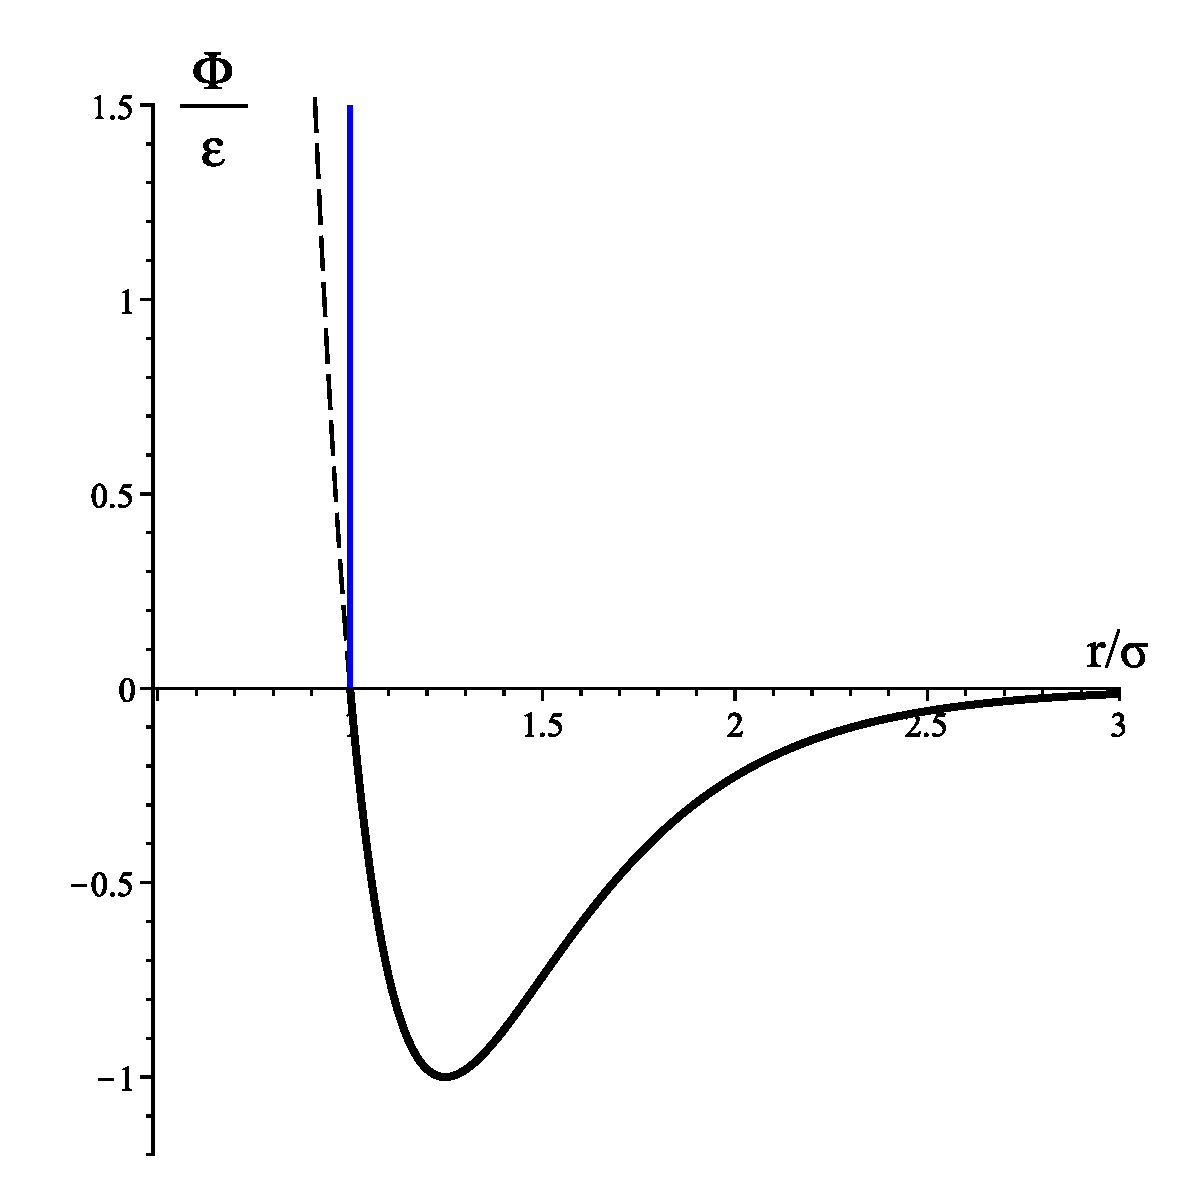
\includegraphics[width=0.45\textwidth,angle=0]{potential} \hfill
		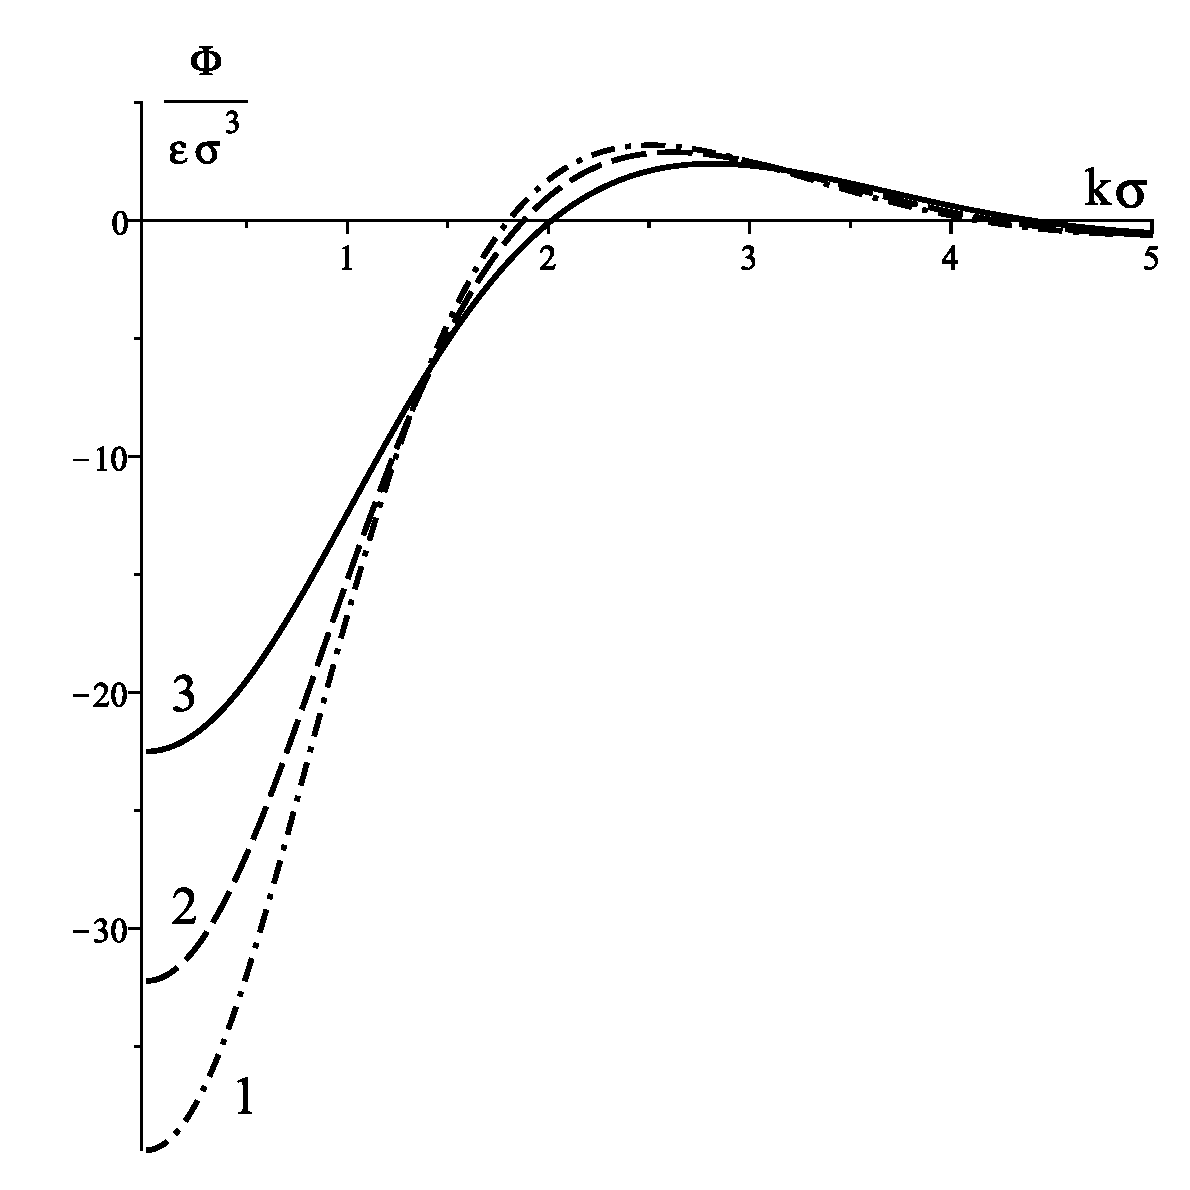
\includegraphics[width=0.45\textwidth,angle=0]{potential-fourier} \\
		\parbox{0.5\textwidth}{\caption*{Fig. 1. Morse potential at $R_0/\alpha = 3.5$.
		}} \hfill
		\parbox{0.45\textwidth}{\caption*{Fig. 2. Fourier transform of a long-range part of interaction potential. The case of Morse potential: 1 - $R_0/\alpha = 2.77,$ 2 - $R_0/\alpha = 3.0,$ 3 - $R_0/\alpha = 3.5$  
		}}
	\end{figure}
	
\end{frame}

\begin{frame}
	\frametitle{Microscopic particle density and collective variables}
	
	\begin{spacing}{1}
		
		\begin{columns}
			\column{0.5\textwidth}
			
			-- Microscopic particle density
			\begin{equation*}
				n(\vb r) = \sum_{j=1}^{N} \delta(\vb r - \vb r_j),
			\end{equation*}
			
			\begin{equation*}
				\int_V n(\vb r) d\vb r = N
			\end{equation*} 
			
			-- Fourier series
			\begin{equation*}
				n(\vb r) = \frac{1}{V} \sum_{\vb k} \hat{\rho}_{\vb k} e^{i\vb k \vb r}
			\end{equation*}
			
			-- Fourier components
			\begin{equation*}
				\label{def:rho_k}
				\hat{\rho}_{\vb k} = \sum_{j=1}^N\exp(-i\vb k \vb r_j), \quad \hat{\rho}_{\vb k = 0} = N. 
			\end{equation*}
			
			
			
			\column{0.45\textwidth}
			
			-- Potential energy of long-range interaction
			\begin{equation*}
				\label{phi_N_via_rho}
				\Phi_N(\vb r^N) = \frac{1}{2V} \sum_{\vb k} \hat{\Phi}_{\vb k} \hat{\rho}_{\vb k} \hat{\rho}_{-\vb k}.
			\end{equation*}
			
			-- Collective variables
			\begin{equation*}
				\hat{\rho}_{\vb k} = \int\rho_{\vb k} J(\rho - \hat{\rho}) ({\rm d}\rho).
			\end{equation*}
			
			-- Jacobian of transformation
			\begin{equation*}
				J(\rho - \hat{\rho}) = \delta(\rho_0 - \hat{\rho}_0) \prod_{\vb k}' \delta(\rho_{\vb k}^c - \hat{\rho}_{\vb k}^c) \delta(\rho_{\vb k}^s - \hat{\rho}_{\vb k}^s),
			\end{equation*}
			
			\begin{equation*}
				({\rm d} \rho) = {\rm d}\rho_0 \prod_{\vb k}' {\rm d}\rho_{\vb k}^c {\rm d}\rho_{\vb k}^s.
			\end{equation*}
			
		\end{columns}
	\end{spacing}
	
\end{frame}

\section{Grand partition function in collective variables}

\begin{frame}
	\frametitle{Grand partition function in collective variables}
	
	\begin{spacing}{1}
		
		\begin{columns}
			\column{0.9\textwidth}
			-- Grand partition function (GPF)
		%	\begin{block}{GPF}
							
			\begin{equation*}
				\Xi = \Xi_0 \int \exp(h\rho_0 - \frac{1}{2V}\sum_{\vb k}
				{\beta\hat{\Phi}_{\vb k}} 
				\rho_{\vb k} \rho_{-\vb k}) \mathfrak{J}(\rho) ({\rm d} \rho)
			\end{equation*}
		%\end{block}
			
			$\Xi_0$ -- GPF of the reference system
			
			$h = \beta(\mu - \mu_0); \quad$
			\hfill \break
			\hfill \break
			-- Jacobian function
			\begin{eqnarray*}
				\label{def:jacobian}
				\mathfrak{J}(\rho) &=& \frac{1}{\Xi_0}\sum_{N=0}^{\infty} \frac{z_0^N}{N!}\int \exp(-\beta\Psi_N(\vb r^N)) J(\rho - \hat{\rho}) {\rm d}{\vb r^N}
				\nonumber\\
				&=& \langle J(\rho - \hat{\rho}) \rangle_{RS}.
			\end{eqnarray*}
			
			
			%\column{0.2\textwidth}
			
			
		\end{columns}
	\end{spacing}
	
\end{frame}

\subsection{Calculation of the Jacobian}

\begin{frame}
	\frametitle{Calculation of the Jacobian}
	
	\begin{spacing}{1}
		
		\begin{columns}
			\column{0.9\textwidth}
			-- Integral representation for $\delta-$functions
			\begin{equation*}
				\delta(\rho_0 - \hat{\rho}_0) \prod_{\vb k}' \delta(\rho_{\vb k}^c - \hat{\rho}_{\vb k}^c) \delta(\rho_{\vb k}^s - \hat{\rho}_{\vb k}^s) = \int \exp(2\pi{\rm i}\sum_{\vb k} (\rho_{\vb k} - \hat{\rho}_{\vb k}) \omega_{\bf k}) ({\rm d} \omega),
			\end{equation*}
			
			-- Cumulant (semi-invariant) expansion
			\begin{equation*}
				\mathfrak{J}(\rho) = \int \exp({\rm i} 2\pi \sum_{\vb k}\rho_{\vb k}\omega_{\vb k}) \tilde{\mathfrak{J}}(\omega) ({\rm d} \omega)
			\end{equation*}
			
			\begin{equation*}
				\tilde{\mathfrak{J}}(\omega) = \left< \exp(-{\rm i}2\pi \sum_{\vb k} \omega_{\vb k}\hat{\rho}_{\vb k}) \right>_{RS} 
				= \frac{(-{\rm i}2\pi)^n}{n!}\sum_{\vb{k}_1,\dotsc,\vb{k}_n}\mathfrak{M}_n(\vb k_1, \dotsc, \vb k_n) \omega_{{\vb k}_1}\dotsc \omega_{{\vb k}_n}
			\end{equation*}
			
			%\column{0.1\textwidth}
			
			
		\end{columns}
	\end{spacing}
	
\end{frame}

\subsection{Cumulants}

\begin{frame}
	\frametitle{Cumulants}
	
	\begin{spacing}{1}
		
		\begin{columns}
			\column{0.9\textwidth}
			-- Definition (general formula):
			\begin{equation*}
				\label{def:cumulant}
				\mathfrak{M}_n(\vb k_1, \dotsc, \vb k_n) = \frac{1}{(-{\rm i}2\pi)^n} 
				\left(
				\frac{\partial^n \ln \tilde{\mathfrak{J}}(\omega)}{\partial\omega_{{\vb k}_1} \dotsc \partial\omega_{{\vb k}_n}}
				\right)_{\omega_{{\vb k}_i}=0}
			\end{equation*}
			
			-- It is shown that any cumulant $\mathfrak{M}_n$ can be represented as
			\begin{equation*}
				\mathfrak M_n(\vb k^n) = \langle N \rangle_0 \mathfrak m_n(\vb k^{n-1}) \delta_{\vb k_1 + \dotsc + \vb k_n}.
			\end{equation*}
			
			$\mathfrak{m}_n$ -- intensive quantity, can be interpreted as $n-$particle structure factor.
			
			\begin{flalign*}
				\rho & = {\langle N \rangle_0}/{V} &
			\end{flalign*} 
			
			
			%\column{0.1\textwidth}
			
			
		\end{columns}
	\end{spacing}
	
\end{frame}

\begin{frame}
	\frametitle{Cumulants expressed via total correlation functions}
	
	\begin{spacing}{1}
		
		\begin{columns}
			\column{0.9\textwidth}
			\begin{equation*}
				\mathfrak{m}_1 = 1.
			\end{equation*}
			\begin{equation*}
				\label{m2}
				\mathfrak m_2(\vb k) = 1 + \rho \hat{h}^{(2)}(\vb k).
			\end{equation*}
			\begin{eqnarray*}
				\label{m3}
				\mathfrak m_3(\vb k_1, \vb k_2) &=& 1 +  \rho \big(\hat{h}^{(2)}(\vb k_1) + \hat{h}^{(2)}(\vb k_2) + \hat{h}^{(2)}(\vb k_1 + \vb k_2) \big)
				\nonumber\\ 
				&& + \rho^2 \hat{h}^{(3)}(\vb k_1, \vb k_2)
			\end{eqnarray*}
			
			\begin{eqnarray*}
				\label{m4}
				&& \mathfrak m_4(\vb k_1, \vb k_2, \vb k_3) =  1 
				\nonumber\\
				&& \quad{} + \rho \bigg(
				\sum_{l = 1}^3 \hat{h}^{(2)}(\vb k_l) +
				\sum_{\vb l = \left\{\substack{1,2 \\ 1,3 \\ 2,3} \right\} }  \hat{h}^{(2)} (\vb k_{l_1} + \vb k_{l_2})
				+ \hat{h}^{(2)} (\vb k_1 + \vb k_2 + \vb k_3)
				\bigg)
				\nonumber \\
				&&  \quad{} + \rho^2 \bigg(
				\sum_{\vb l = \left\{\substack{1,2 \\ 1,3 \\ 2,3 }\right\} }
				\hat{h}^{(3)}(\vb k_{l_1}, \vb k_{l_2})
				+ \sum_{\vb l = \left\{\substack{1,2,3 \\ 1,3,2 \\ 2,3,1}\right\} }
				\hat{h}^{(3)}(\vb k_{l_1} + \vb k_{l_2}, \vb k_{l_3})
				\bigg)
				\nonumber\\
				&& \quad{} + \rho^3 \hat{h}^{(4)} (\vb k_1, \vb k_2, \vb k_3)
			\end{eqnarray*}
			
			
			\column{0.1\textwidth}
			
			
		\end{columns}
	\end{spacing}
	
\end{frame}

\begin{frame}
	\frametitle{Bell numbers and Stirling numbers of $2^{nd}$ type in $\mathfrak{m}_n$}
	
	\begin{spacing}{1}
		
		\begin{columns}
			\column{0.9\textwidth}
			-- Bell number $B_n$ -- the total number of all terms contributing to $\mathfrak{m}_n$
			
			See \url{https://en.wikipedia.org/wiki/Bell_number}
			
			\hfill{} \break
			
			-- Stirling number of the second kind $S(n, k)$ -- the number of terms at the $k-$th power in $\rho$
			
			{ } \url{https://en.wikipedia.org/wiki/Stirling_numbers_of_the_second_kind}
			
			
			%\column{0.1\textwidth}
			
			
		\end{columns}
	\end{spacing}
	
\end{frame}

\subsection{Hierarchy of total correlation functions}

\begin{frame}
	\frametitle{Total correlation functions}
	
	%\begin{spacing}{1}
		
		%\begin{columns}
		%	\column{0.9\textwidth}
		-- $n$-particle distribution function
		\begin{equation*}
			\label{def:g_n}
			g^{(n)}(\vb{r}^n)=\frac{\rho^{(n)}(\vb{r}_1,\dotsc,\vb{r}_n)}{\prod_{i=1}^{n}\rho^{(1)}(\vb{r}_i)}
		\end{equation*}
		
		-- $n$-particle density
		\begin{eqnarray*}
			\label{def:rho_n}
			\rho^{(n)}(\vb r^n) = \frac{1}{\Xi}\sum_{N=n}^{\infty} \frac{z^N}{(N-n)!} \int\exp(-\beta U_N) d\vb r^{(N-n)}
		\end{eqnarray*}
		
		\textbf{Hierarchy of total correlation functions:}
		\hfill{} \break
		
		$n=1:$
		\begin{equation*}
			h^{(1)}(\vb{r}) = g^{(1)}(\vb{r}) = 1.
		\end{equation*}
		
		$n=2$ - pair (radial) correlation function
		\begin{equation*}
			\label{def:pair_corr_func}
			h^{(2)}(\vb{r}_1,\vb{r}_2) = g^{(2)}(\vb{r}_1,\vb{r}_2) - 1
		\end{equation*}
		
		%	\column{0.1\textwidth}
		
		
		%\end{columns}
	%\end{spacing}
	
\end{frame}

\begin{frame}
	\frametitle{Total correlation functions}
	
	\begin{spacing}{1}
		
		%\begin{columns}
		%	\column{0.9\textwidth}
		
		$n=3:$
		\begin{eqnarray*}
			h^{(3)}(\vb{r}_1 ,\vb{r}_2, \vb{r}_3) &=& g^{(3)}(\vb{r}_1, \vb{r}_2, \vb{r}_3) - g^{(2)}(\vb{r}_1, \vb{r}_2) 
			\nonumber\\
			&&-g^{(2)}(\vb{r}_1,\vb{r}_3) -  g^{(2)}(\vb{r}_2,\vb{r}_3) +2.
		\end{eqnarray*}
		
		$n=4:$
		\begin{eqnarray*}
			h^{(4)}(1,2,3,4) &=& g^{(4)}(1,2,3,4) 
			- \sum_{\vb l = \left\{\substack{1,2,3,4 \\ 1,2,4,3 \\ 1,3,4,2 \\ 2,3,4,1}\right\} }g^{(3)}(l_1,l_2,l_3) g^{(1)}(l_4) 
			\nonumber\\
			&&-\sum_{\vb l = \left\{ \substack{1,2,3,4 \\ 1,3,2,4 \\ 1,4,2,3} \right\}}g^{(2)}(l_1,l_2) g^{(2)}(l_3,l_4)
			\nonumber\\
			&& + 2\sum_{\vb l = \left\{\substack{1,2,3,4 \\ 1,3,2,4 \\ 1,4,2,3 \\ 2,3,1,4 \\ 2,4,1,3 \\ 3,4,1,2} \right\}} g^{(2)}(l_1,l_2)g^{(1)}(l_3) g^{(1)}(l_4) 
			\nonumber\\
			&&-6g^{(1)}(1) g^{(1)}(2)g^{(1)}(3) g^{(1)}(4).
		\end{eqnarray*}
		
		%	\column{0.1\textwidth}
		
		
		%\end{columns}
	\end{spacing}
	
\end{frame}

\begin{frame}
	\frametitle{Total correlation functions: definitions}
	
	%\begin{spacing}{1}
		
		Phil Attard, J. Chem. Phys. 93 (1990); doi: 10.1063/1.459402
		
		%\begin{columns}
		%	\column{0.9\textwidth}
		\begin{figure}[htbp]
			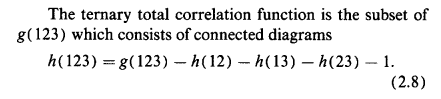
\includegraphics[width=0.45\textwidth,angle=0]{attard-triplet-correlation-function} \hfill
			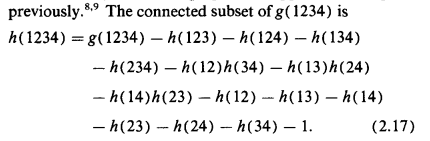
\includegraphics[width=0.45\textwidth,angle=0]{attard-triplet-correlation-function-quartic} \\
			%\parbox{0.1\textwidth}{\caption*{}} \hfill
			%\parbox{0.1\textwidth}{\caption*{}}
		\end{figure}
		
		\hfill
		
		J.A.~Hernando, Phys. Rev. A, 33, (1986); doi: 10.1103/PhysRevA.33.1338
		
		\begin{figure}[htbp]
			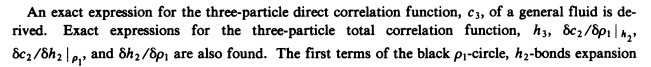
\includegraphics[width=0.55\textwidth,angle=0]{hernando-abstract2} \hfill
			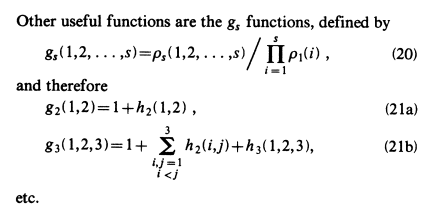
\includegraphics[width=0.4\textwidth,angle=0]{hernando-corr-func-def} \\
			%\parbox{0.5\textwidth}{\caption*{}} \hfill
			%\parbox{0.5\textwidth}{\caption*{}}
		\end{figure}
		
		
		
		%	\column{0.1\textwidth}
		
		
		%\end{columns}
	%\end{spacing}
	
\end{frame}

\begin{frame}
	\frametitle{Fourier transforms for Total correlation functions}
	
	\begin{spacing}{1}
		
		%\begin{columns}
		%	\column{0.9\textwidth}
		-- Fourier transformation
		\begin{eqnarray*}
			&&\hat{h}^{(n)}(\vb{k}_1,\dotsc, \vb{k}_n) 
			\\
			&&= \int \exp(-{\rm i}\vb{k}_1\vb{r}_1 - \dotsc - {\rm i}\vb{k}_n\vb{r}_n) h^{(n)}(\vb{r}_1, \dotsc, \vb{r}_n) d\vb{r}_1\dotsc d\vb{r}_n
			\nonumber
		\end{eqnarray*}
		
		
		-- The following property holds for total correlation functions
		\begin{equation*}
			\frac{1}{V}\hat{h}^{(n)} (\vb{k}^n) = \hat{h}^{(n)} (\vb{k}_1, \dotsc, \vb{k}_{n-1}) 
			\delta_{\vb{k}_1+\dotsc + \vb{k}_n}
		\end{equation*}
		
		
		%	\column{0.1\textwidth}
		
		
		%\end{columns}
	\end{spacing}
	
\end{frame}

\begin{frame}
	\frametitle{Recurrence relations for Total correlation functions}
	
	\begin{spacing}{1}
		
		%\begin{columns}
		%	\column{0.9\textwidth}
		-- Recurrence relations [Schofield, Proc. Phys. Soc., \textbf{88} (1966)]
		
		\begin{eqnarray*}
			\label{recur_g}
			&&\frac{\partial (\rho^n g^{(n)})}{\partial\rho} \bigg|_T 
			= 
			\\
			&& = \frac{n\rho^{n-1}g^{(n)} + \rho^n \int \{g^{(n+1)}(\vb r_1, \dots, \vb r_{n+1}) - g^{(n)}(\vb r_1, \dots, \vb r_n)\} {\rm d} \vb r_{n+1}}
			{1 + \rho\int \{g^2(\vb r_1, \vb r_2) - 1\} {\rm d} \vb r_1}
			\nonumber
		\end{eqnarray*}
		
		-- Explicit relationship for $\hat{h}^{(3)}$ via $\hat{h}^{(2)}$:
		\begin{equation*}
			\label{recur_h3_h2}
			\hat{h}^{(3)}(k, -k) = 2 \hat{h}^{(2)}(0)\hat{h}^{(2)}(k) + \frac{\partial \hat{h}^{(2)}(k)}{\partial\rho}(1 + \rho\hat{h}^{(2)}(0)).
		\end{equation*}
		
		-- Explicity relationship for $\hat{h}^{(4)}$ via $\hat{h}^{(3)}$:
		\begin{eqnarray*}
			\label{recur_h4_h3}
			\hat{h}^{(4)}(k, -k, 0) &=& 3\hat{h}^{(2)}(0)\hat{h}^{(3)}(k, -k) 
			\nonumber\\
			&+& \frac{\partial \hat{h}^{(3)}(k, -k)} {\partial \rho} (1 + \rho\hat{h}^{(2)}(0))
		\end{eqnarray*}
		
		
		%	\column{0.1\textwidth}
		
		
		%\end{columns}
	\end{spacing}
	
\end{frame}

\begin{frame}
	\frametitle{Recurrence relations for cumulants}
	
	\begin{spacing}{1}
		
		\begin{columns}
			\column{0.9\textwidth}
		
		-- Explicit relationship for $\mathfrak{m}_{3}$ via $\mathfrak{m}_{2}$:
		\begin{equation*}
			\label{recur_m3_m2}
			\mathfrak{m}_3(k, -k) = \mathfrak{m}_2(0) 
			\left[
			\mathfrak{m}_2(k) + \eta\frac{\partial\mathfrak{m}_2(k)}{\partial\eta}
			\right],
		\end{equation*}
		
		
		-- Explicity relationship for $\mathfrak{m}_{4}$ via $\mathfrak{m}_{3}$:
				
		\begin{eqnarray*}
			\label{recur_m4_m2}
			\mathfrak{m}_4(k, -k, 0) &=& \mathfrak{m}_2(0) 
			\left[
			\mathfrak{m}_2(k)\mathfrak{m}_2(0) + 3\eta\mathfrak{m}_2(0)\frac{\partial\mathfrak{m}_2(k)}{\partial\eta}
			\right.
			\nonumber\\
			&& \left. 
			+ \eta\mathfrak{m}_2(k)\frac{\partial\mathfrak{m}_2(0)}{\partial\eta} 
			+ \eta^2\frac{\partial\mathfrak{m}_2(0)}{\partial\eta} \frac{\partial\mathfrak{m}_2(k)}{\partial\eta}
			\right.
			\nonumber\\
			&& \left.
			+ \eta^2\mathfrak{m}_2(0)\frac{\partial^2\mathfrak{m}_2(k)}{\partial\eta^2}
			\right]
		\end{eqnarray*}
		
		-- $\eta$ is packing fraction
		\begin{flalign*}
			\eta & = \frac{\pi}{6} \frac{\langle N \rangle_0}{V}\sigma^3 &
		\end{flalign*}
		
		
		%	\column{0.1\textwidth}
		
		
		\end{columns}
	\end{spacing}
	
\end{frame}

\begin{frame}
	\frametitle{Cumulants for the hard-sphere system}
	
	\begin{spacing}{1}
		
		%\begin{columns}
		%	\column{0.9\textwidth}
		
		-- Given the equation of state for the hard-sphere system in the form:
		\begin{equation*}
			\frac{PV}{NkT} = f(\eta)
		\end{equation*}
		
		
		-- Second cumulant $\mathfrak{m}_{2}$ is found as:
		\begin{equation*}
			\mathfrak{m}_2 = S(0) = kT\left(\frac{\partial \rho}{\partial P}\right)_T.
		\end{equation*}
		
		\begin{equation*}
			\frac{1}{\mathfrak{m}_2} = f(\eta) + \eta \frac{\partial f(\eta)}{\partial \eta}.
		\end{equation*}
		
		-- In Carnahan-Starling approximation:
		\begin{equation*}
			\mathfrak{m}_2 = \frac{(1-\eta)^4}{(1+2\eta)^2 - 4\eta^3 + \eta^4},
			\nonumber
		\end{equation*}
		
		
		%	\column{0.1\textwidth}
		
		
		%\end{columns}
	\end{spacing}
	
\end{frame}

\begin{frame}
	\frametitle{Graphical representations for $\mathfrak{m}_2$}
	
	\begin{spacing}{1}
		
		%\begin{columns}
		%	\column{0.9\textwidth}
		\begin{figure}[htbp]
			\includegraphics[width=0.45\textwidth,angle=0]{M2_as_function_of_k_at_different_eta2} \hfill
			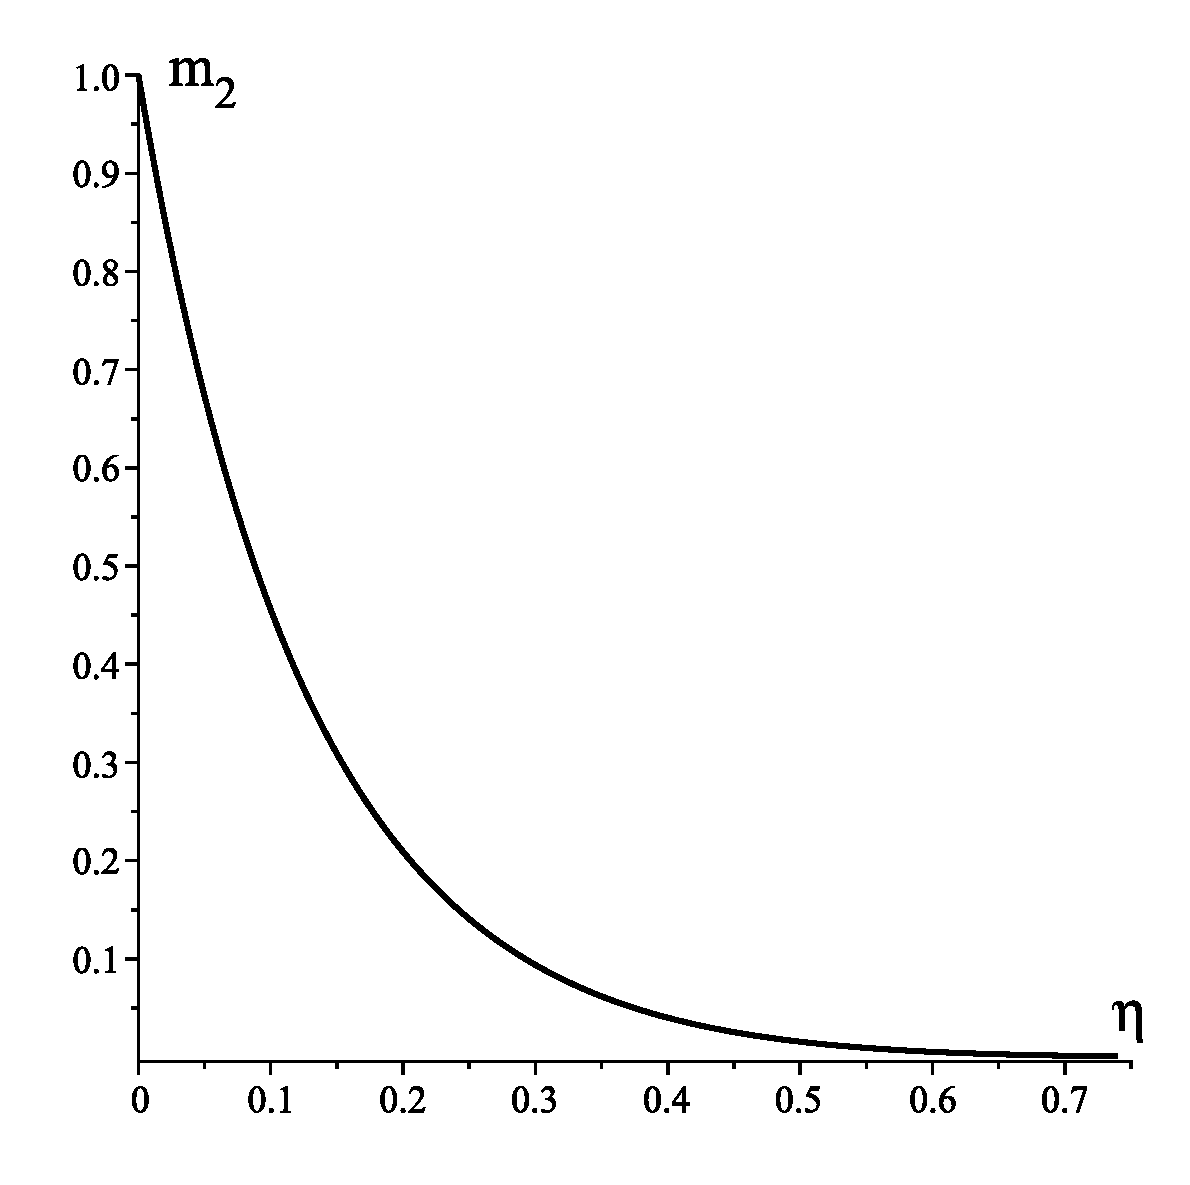
\includegraphics[width=0.45\textwidth,angle=0]{M2_as_function_of_eta_at_k_equals_0} \\
			\parbox{0.5\textwidth}{\caption*{\label{m2_vs_k} Fig. 3. Cumulant $\mathfrak{m}_2$ as a function of $k\sigma$ at different values of packing fraction $\eta$. 1 - $\eta = 0.05$, 2 - $\eta=0.1$, 3 - $\eta = 0.15$, and 4 - $\eta=0.2$.
			}} \hfill
			\parbox{0.45\textwidth}{\caption*{\label{m2_vs_eta} Fig. 4. Cumulant $\mathfrak{m}_2$ as a function of packing fraction $\eta$ at $\vb k = 0$
			}}
		\end{figure}
		
		
		%	\column{0.1\textwidth}
		
		
		%\end{columns}
	\end{spacing}
	
\end{frame}

\begin{frame}
	\frametitle{Graphical representations for $\mathfrak{m}_4$}
	
	\begin{spacing}{1}
		
		%\begin{columns}
		%	\column{0.9\textwidth}
		\begin{figure}[htbp]
			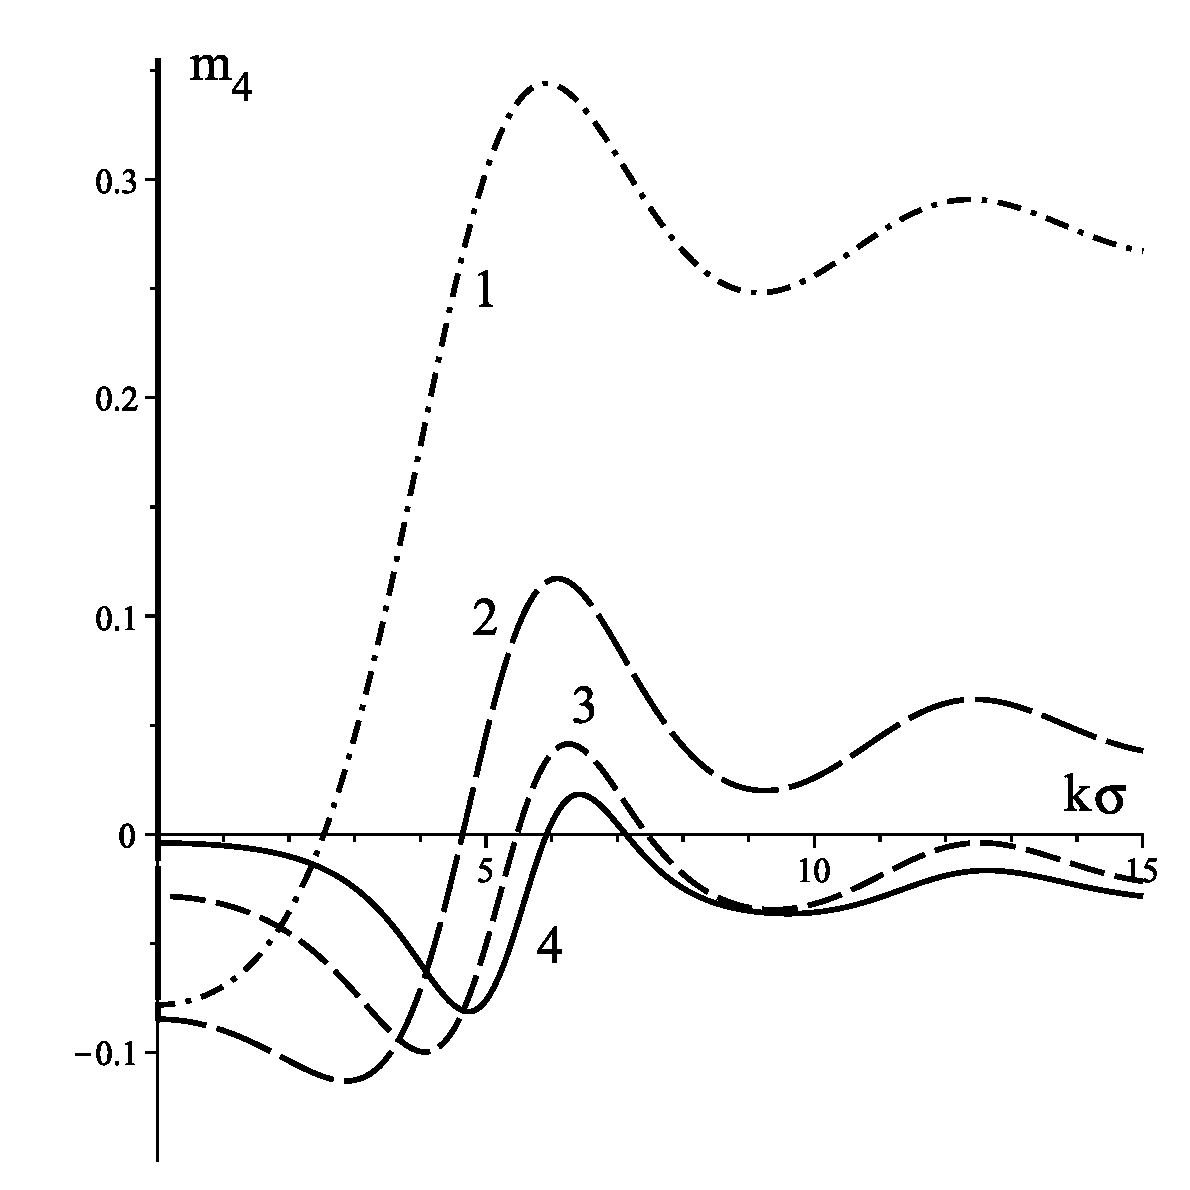
\includegraphics[width=0.45\textwidth,angle=0]{M4_as_function_of_k_at_different_eta} \hfill
			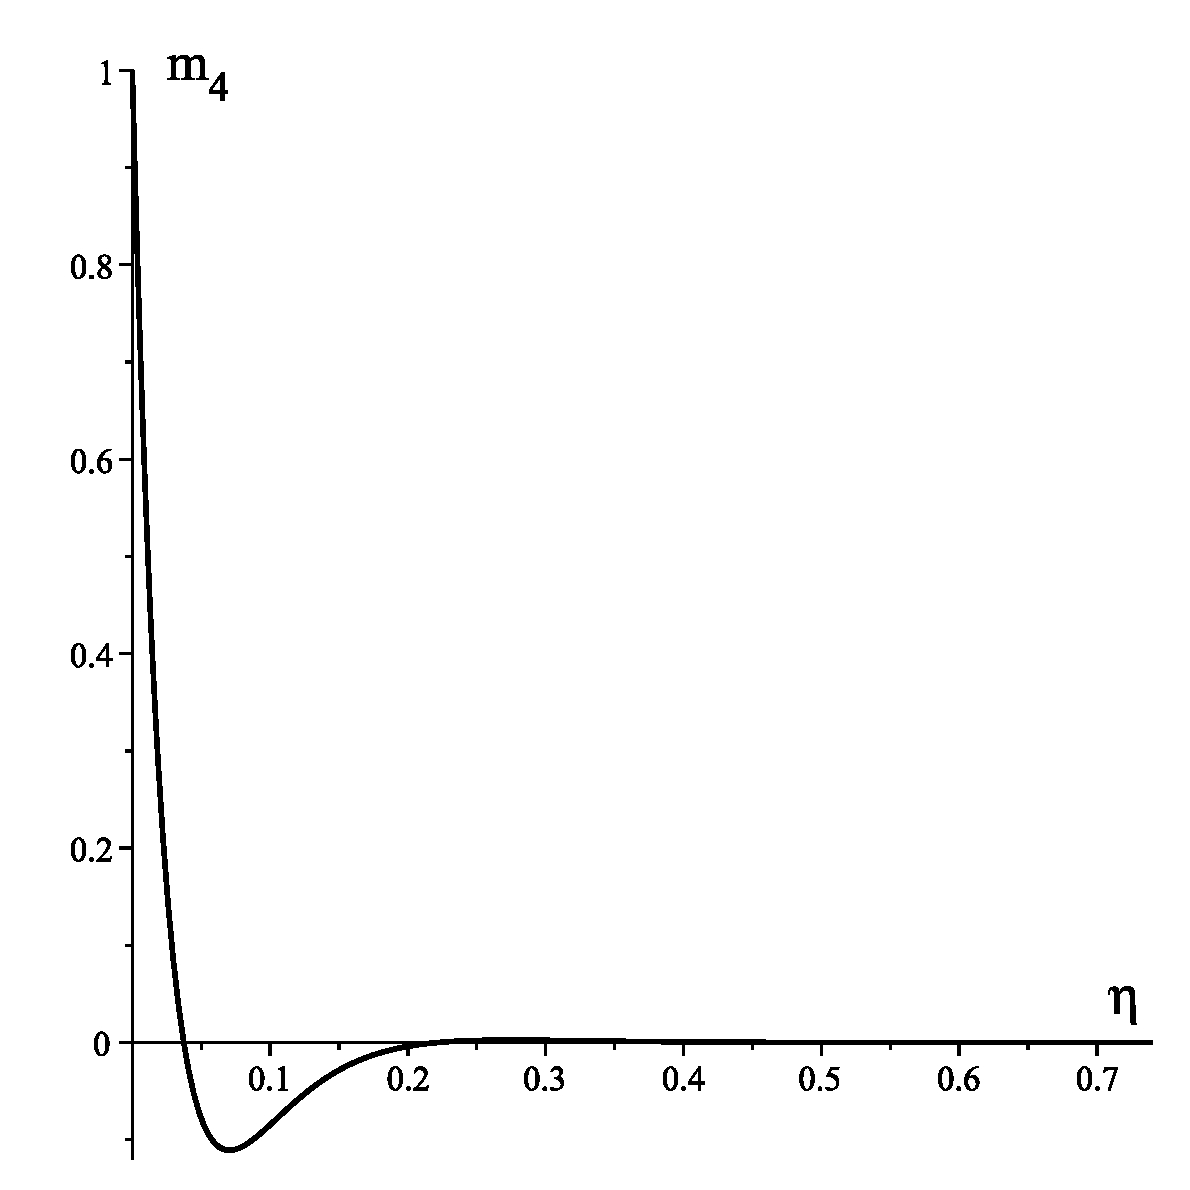
\includegraphics[width=0.45\textwidth,angle=0]{M4_as_function_of_eta_at_k_equals_0} \\
			\parbox{0.5\textwidth}{\caption*{\label{m4_vs_k} Fig. 5. Cumulant $\mathfrak{m}_4$ as a function of $k\sigma$ at different values of packing fraction $\eta$. 1 - $\eta = 0.05$, 2 - $\eta=0.1$, 3 - $\eta = 0.15$, and 4 - $\eta=0.2$.
			}} \hfill
			\parbox{0.45\textwidth}{\caption*{\label{m4_vs_eta} Fig. 6. Cumulant $\mathfrak{m}_4$ as a function of packing fraction $\eta$ at $\vb k = 0$
			}}
		\end{figure}
		
		
		
		%	\column{0.1\textwidth}
		
		
		%\end{columns}
	\end{spacing}
	
\end{frame}

\begin{frame}
	\frametitle{Functional form for Grand partition function}
	
	\begin{spacing}{1}
		
		%\begin{columns}
		%	\column{0.9\textwidth}
		
		\begin{eqnarray*}
			\label{gpf_1}
			&&\Xi = \Xi_0 \int \exp \left[h \rho_0 - \frac{1}{2V}
			\sum\limits_{\bf k} {\beta\hat{\Phi}_{\vb k}} \rho_{\bf k}\rho_{-{\bf k}} \right]
			\\
			&&
			\quad{}\times
			\exp \left(i2\pi \sum\limits_{\bf k} \omega_{\bf k} \rho_{\bf k} \right.
			\nonumber\\
			&& \quad{} + \left. \sum_{n\ge 1} \frac{(-i2\pi)^n}{n!}\sum_{\vb{k}_1,\dotsc,\vb{k}_n} {\mathfrak M}_n(\vb{k}_1,\dotsc,\vb{k}_n) \omega_{\vb k_1}\dotsc\omega_{\vb{k}_n} \right) 
			\nonumber\\
			&&
			\quad{}\times ({\rm d}\omega) ({\rm d}\rho) 
			\nonumber
		\end{eqnarray*}
		
		
		%	\column{0.1\textwidth}
		
		
		%\end{columns}
	\end{spacing}
	
\end{frame}

\begin{frame}
	\frametitle{Functional form for Grand partition function}
	
	\begin{spacing}{1}
		
		\begin{columns}
		\column{0.9\textwidth}
				
		{\it Approximation 1.} The expression for $\Xi$ is restricted to $\mathfrak{M}_4$.
		
		$\quad \quad$ NB: $\mathfrak{m}_4 < 0$ only for $0.04 < \eta < 0.22$
		
		\hfill
		
		{\it Approximation 2.} The dependence of cumulants $\mathfrak{M}_n$ on the wave vectors $\vb k_i$ is neglected, except for the dependence via $\delta$-functions
		\begin{equation*}
			\mathfrak{M}_n({\vb k}^n) \approx \mathfrak{M}_n(0^n) \delta_{\vb{k}_1 + \dotsc + \vb{k}_n}
		\end{equation*}
		
		\hfill
		
		{\it{Approximation 3.}} Integration over $\rho_{\vb k}$ with $k > B$ is carried out with Gaussian measure, $B$ being a cutoff parameter, e.g. following from condition $\hat{\Phi}_B = 0$.
		
		
		%	\column{0.1\textwidth}
		
		
		\end{columns}
	\end{spacing}
	
\end{frame}

\begin{frame}
	\frametitle{Functional form for Grand partition function}
	
	%\begin{spacing}{1}
		
		%\begin{columns}
		%	\column{0.9\textwidth}
		
		\begin{equation*}
			\label{Xi_as_prod}
			\Xi = \Xi_0\Xi_G\Xi_L
		\end{equation*}
		
		\begin{eqnarray*}
			\label{Xi_L_1}
			\Xi_L & \propto & {\rm e}^{\tilde{\mathfrak{M}}_0}
			\int \exp\left(
			\mu^* \rho_0 - \frac{1}{2} \sum_{\substack{\vb k \\ k \leq B}} d(k) \rho_{\vb k} \rho_{-\vb k} 
			\right.\\
			&& -\left. \frac{a_4}{4! N_B} \sum_{\substack{\vb k_1, \dotsc, \vb k_4 \\ k_i \leq B}} \rho_{\vb k_1} \dotsc \rho_{\vb k_4} \delta_{\vb{k}_1 + \dotsc + \vb{k}_4} \right) ({\rm d} \rho)^{N_B}
			\nonumber
		\end{eqnarray*}
		
		Notation:
		\begin{equation*}
			d(k) = a_2 + \frac{\beta\hat{\Phi}_{\vb k}}{V},
		\end{equation*}
		\begin{equation*}
			 \mu^* = \beta(\mu - \mu_0) + \frac{\mathfrak{m}_3}{\mathfrak{m_4}} + 
			 \frac{\langle N \rangle_0}{V}\beta\hat{\Phi}_0 
			 \left(
			 	1 + \frac{\mathfrak{m}_2 \mathfrak{m}_3}{\abs{\mathfrak{m}_4}} + \frac{\mathfrak{m}_3^3}{3\mathfrak{m}_4^2}
			 \right)
		\end{equation*}
		\begin{equation*}
			\label{tilde_frak_M0}
			\tilde{\frak M}_0 = \left(\beta(\mu - \mu_0) + \frac{\mathfrak{m}_3}{\mathfrak{m}_4}\right)
			\left(
			1 + \frac{\mathfrak{m}_2 \mathfrak{m}_3}{\abs{\mathfrak{m}_4}} + \frac{\mathfrak{m}_3^3}{3\mathfrak{m}_4^2}
			\right)
		\end{equation*}
		
		
		%	\column{0.1\textwidth}
		
		
		%\end{columns}
	%\end{spacing}
	
\end{frame}

\begin{frame}
	\frametitle{Coefficients of the effective hamiltonian}
	
	\begin{spacing}{1}
		
		%\begin{columns}
		%	\column{0.9\textwidth}
		\begin{figure}[htbp]
			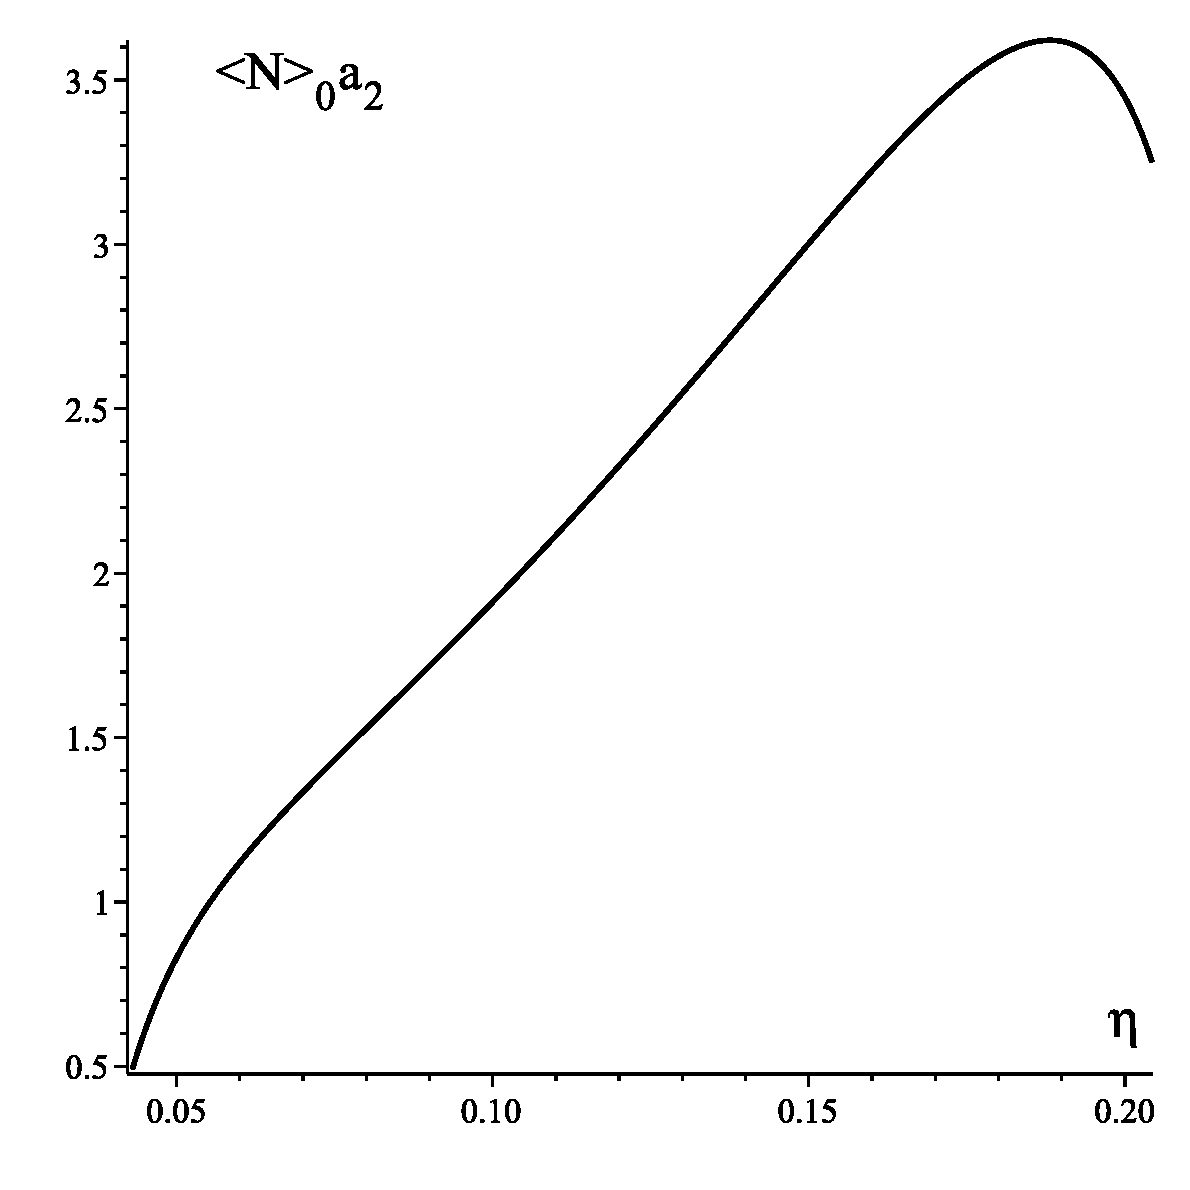
\includegraphics[width=0.45\textwidth,angle=0]{a2_as_function_of_eta} \hfill
			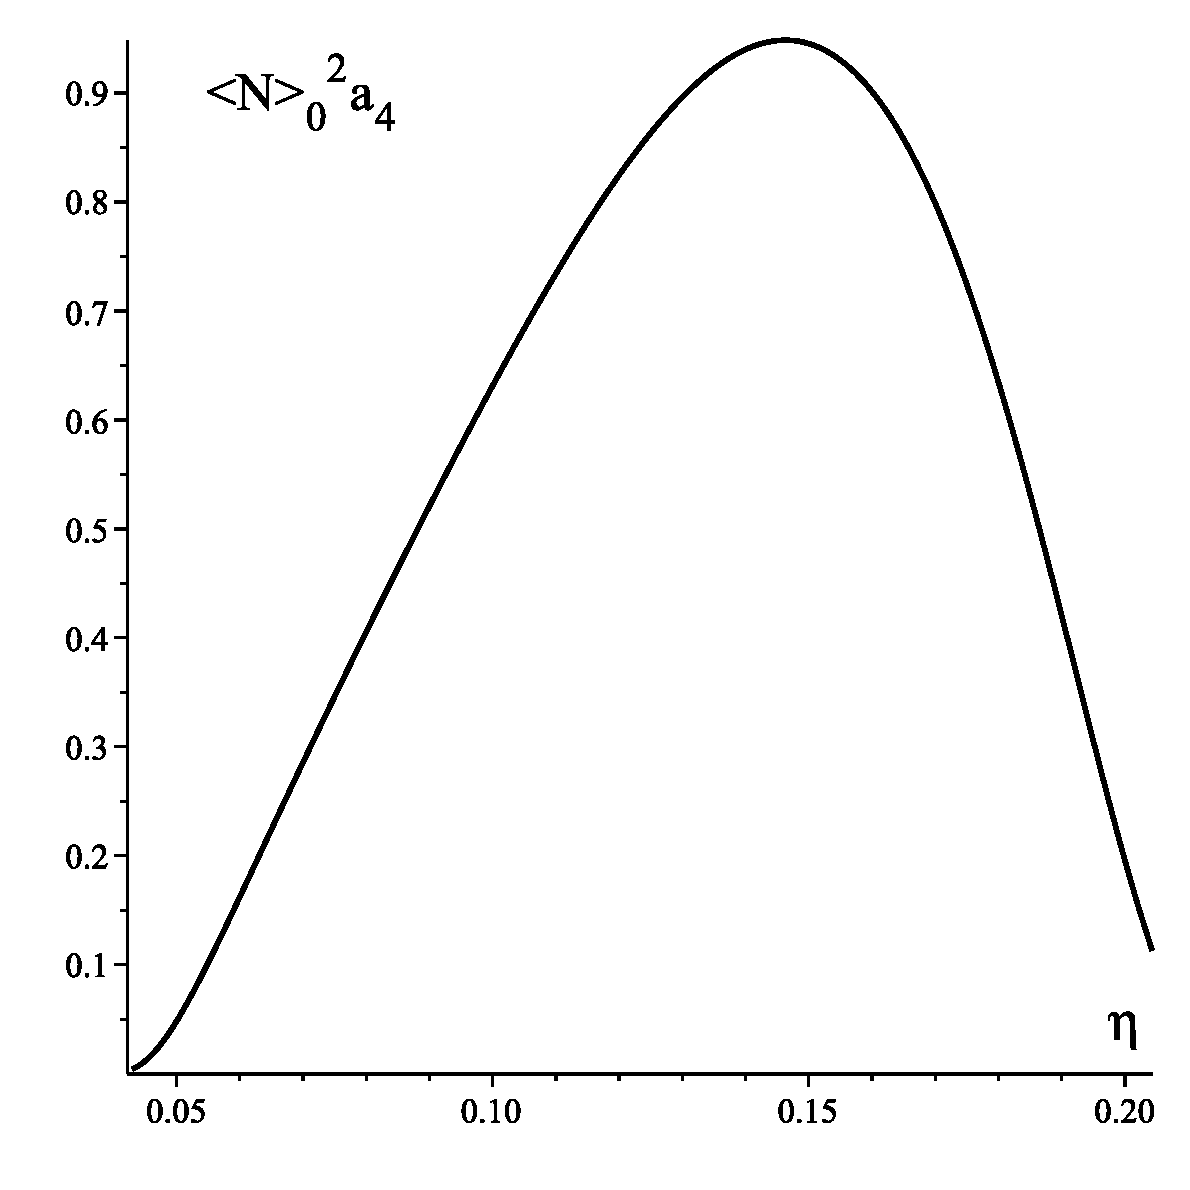
\includegraphics[width=0.45\textwidth,angle=0]{a4_as_function_of_eta} \\
			\parbox{0.5\textwidth}{\caption*{Fig. 7.}} \hfill
			\parbox{0.45\textwidth}{\caption*{Fig. 8}}
		\end{figure}
		
		
		
		%	\column{0.1\textwidth}
		
		
		%\end{columns}
	\end{spacing}
	
\end{frame}

\section{Critical point in mean-field approximation}

\begin{frame}
	\frametitle{Critical point in mean-field approximation}
	
	\begin{spacing}{1}
		
		\begin{columns}
			\column{0.9\textwidth}
		
		\begin{equation*}
			\Xi_L^{(1)} = \int \exp(\mu^*\rho_0 -\frac{d(0)}{2} \rho_0^2 - \frac{a_4}{4!N_B} \rho_0^4) {\rm d} \rho_0.
		\end{equation*}
		
		Since $d(0) \propto \langle N \rangle_0$ and $a_4 \propto \langle N \rangle_0^2$, perform substitution of variables 
		$\rho = \langle N \rangle_0 \rho_0'$
		
		
		\begin{equation*}
			\Xi_L^{(1)} = \langle N \rangle_0 \int \exp[\langle N \rangle_0 E(\rho'_0)] {\rm d} \rho'_0
		\end{equation*}
		
		\hfill
		
		\begin{equation*}
			E(\rho'_0) = \mu^*\rho_0' - \frac{d'(0)}{2} {\rho'}_0^2 - \frac{a'_4}{4!}{\rho'}_0^4,
		\end{equation*}
		\begin{equation*}
			d'(0) = \langle N \rangle_0 d(0) = a'_2 + \frac{6}{\pi}\eta \frac{\varepsilon}{k_BT} \frac{\hat{\Phi}_0}{\varepsilon\sigma^3}.
		\end{equation*}
		\begin{equation*}
			a'_2 = \langle N \rangle_0 a_2, \quad a'_4 = \frac{\langle N \rangle_0}{N_B} \langle N \rangle_0^2 a_4
		\end{equation*}
		
		
		
		%\column{0.1\textwidth}
		
		
		\end{columns}
	\end{spacing}
	
\end{frame}

\begin{frame}
	\frametitle{Critical point in mean-field approximation}
	
	\begin{spacing}{1}
		
		\begin{columns}
			\column{0.9\textwidth}
			
			-- Applying the steepest-descent method
			
			\begin{equation*}
				\label{mf:Xi_L_1}
				\Xi_L^{(1)} = \langle N \rangle_0 \exp(\langle N \rangle_0 E(\rho_{0,{\rm max}}))
			\end{equation*}
			
			-- where $\rho_{0, {\rm max}}$ maximizes $E(\rho_0)$
			\begin{equation*}
				\frac{\partial E}{\partial \rho'_0} = 0; \quad \frac{\partial^2 E}{\partial {\rho'}_0^2} < 0.
			\end{equation*}
			
			-- in explicit form
			\begin{equation*}
				\label{eq_rho_mean_field}
				\mu^*-d'(0)\rho_0 - \frac{a'_4}{3!}{\rho'}_0^3 = 0,
			\end{equation*}
			\begin{equation*}
				-d'(0) - \frac{a'_4}{2}{\rho'}_0^2 < 0.
			\end{equation*}
			
			%\column{0.1\textwidth}
			
			
		\end{columns}
	\end{spacing}
	
\end{frame}

\begin{frame}
	\frametitle{Critical point in mean-field approximation}
	
	\begin{spacing}{1}
		
		\begin{columns}
			\column{0.45\textwidth}
			
			-- First conditions for critical point to exist
			\begin{equation*}
				\mu^* = 0
			\end{equation*}
			
			-- Solutions for $\rho_{\rm max}$ at $\mu^* = 0$
			$$
			\rho_{01, {\rm max}} = 0; \quad \rho_{02,03, {\rm max}} = \pm\sqrt{-\frac{3!d'(0)}{a'_4}}
			$$ 
			
			-- Second condition for critical point to exist
			\begin{equation*}
				d(0) = 0
			\end{equation*}
			
			\column{0.5\textwidth}
			
			-- Thermodynamic expression for the average number of particles
			\begin{equation*}
				\left(\frac{\partial \ln\Xi}{\partial (\beta\mu)}\right)_{T,V} = \langle N \rangle.
			\end{equation*}
			
			-- This gives rise to
			\begin{equation*}
				\langle N \rangle_0
				\left(
				\mathfrak{m}_1 + \frac{\mathfrak{m}_2 \mathfrak{m}_3}{\abs{\mathfrak{m}_4}} + \frac{\mathfrak{m}_3^3}{3\mathfrak{m}_4^2}  + \rho_0^{\rm{max}}
				\right) 
				= \langle N \rangle.
			\end{equation*}
			
			-- Third condition that we use to get the critical point coordinates
			\begin{equation*}
				\langle N \rangle_0 = \langle N \rangle.
			\end{equation*}
			
			-- This leads to
			\begin{equation*}
				\rho_0^{\rm{max}} = - \left(\frac{\mathfrak{m}_2 \mathfrak{m}_3}{\abs{\mathfrak{m}_4}} + \frac{\mathfrak{m}_3^3}{3\mathfrak{m}_4^2}\right) = 0.
			\end{equation*}
			
		\end{columns}
	\end{spacing}
	
\end{frame}

\begin{frame}
	\frametitle{Critical point in mean-field approximation}
	
	\begin{spacing}{1}
		
		\begin{columns}
			\column{0.3\textwidth}
			
			-- Condition $\mu^* = 0:$
			
			\column{0.65\textwidth}
			
			\begin{flalign*}
				\beta(\mu - \mu_0) + \frac{\mathfrak{m}_3}{\mathfrak{m_4}} + 
				\frac{\langle N \rangle_0}{V}\beta\hat{\Phi}_0 
				\left(
				1 + \frac{\mathfrak{m}_2 \mathfrak{m}_3}{\abs{\mathfrak{m}_4}} + \frac{\mathfrak{m}_3^3}{3\mathfrak{m}_4^2}
				\right) & = 0 &
			\end{flalign*}
			
			
		\end{columns}
		
		\begin{columns}
			\column{0.3\textwidth}
			
			-- Condition $d(0) = 0:$
			
			\column{0.65\textwidth}
			
			\begin{flalign*}
				a'_2 + \frac{6\eta}{\pi} \frac{1}{T^*} \frac{\hat{\Phi}_0}{\varepsilon\sigma^3} & = 0 &
			\end{flalign*}
			
			
		\end{columns}
		
		\begin{columns}
			\column{0.3\textwidth}
			
			-- Condition $\langle N \rangle_0 = \langle N \rangle:$
			
			\column{0.65\textwidth}
			
			\begin{flalign*}
				\frac{\mathfrak{m}_2 \mathfrak{m}_3}{\abs{\mathfrak{m}_4}} + \frac{\mathfrak{m}_3^3}{3\mathfrak{m}_4^2} & = 0. &
			\end{flalign*}
			
		\end{columns}
		
		\hfill
		
		\hrule
		\begin{columns}
			
			\column{0.25\textwidth}
		

		
		\begin{equation*}
			\eta_c = 0.13044 \quad (\rho^*_c = 0.24913)
		\end{equation*}
		\begin{equation*}
			T^*_c = -\frac{6\eta_c}{\pi a'_2} \frac{\hat{\Phi}_0}{\varepsilon\sigma^3}
		\end{equation*}
		\begin{equation*}
			\beta(\mu_c - \mu_0) = -\frac{\rho^*_c}{T^*_c} \frac{\hat{\Phi}_0}{\varepsilon\sigma^3} = a'_2
		\end{equation*}
		
		\column{0.1\textwidth}
		
		\column{0.35\textwidth}
		
		-- Notation
		\begin{equation*}
			\rho^* = \frac{\langle N \rangle}{V} \sigma^3
		\end{equation*}
		$$ \eta = \frac{\pi}{6} \frac{\langle N \rangle}{V} \sigma^3 = \frac{\pi}{6}\rho^* $$
		\begin{equation*}
			T^* = \frac{kT}{\varepsilon}
		\end{equation*}
		
		\end{columns}
		
		
	\end{spacing}
	
\end{frame}

\begin{frame}
	\frametitle{Critical point in mean-field approximation}
	
	\begin{table}[h]
		\caption*{Table I. Critical values of temperature and chemical potential for different parameters $R_0/\alpha$.}
		\begin{center}
			\begin{tabular}{|c|c|c|c|}
				%\begin{tabular}{cccccccccc}
				\hline
				$R_0/\alpha$ \quad & $T^*_c$ \quad & $\beta(\mu_c - \mu_0)$ \quad & $\beta\mu^{\rm{ex}}_c$ \quad \quad \\
				\hline
				2.0  & 9.592 & 2.6699 & 4.0342 \\
				2.5  & 4.931 & 2.6228 & 3.9872 \\
				3.0  & 3.111 & 2.5812 & 3.9456 \\
				3.5  & 2.202 & 2.5453 & 3.9097 \\
				4.0  & 1.677 & 2.5143 & 3.8787 \\
				4.5  & 1.342 & 2.4877 & 3.8520 \\
				5.0  & 1.112 & 2.4645 & 3.8289 \\
				5.5  & 0.946 & 2.4444 & 3.8088 \\
				6.0  & 0.821 & 2.4268 & 3.7911 \\
				\hline
			\end{tabular}
		\end{center}
		\label{tab:critical_chem_potential}
	\end{table}
	
	\begin{columns}
		\column{0.2\textwidth}
		$$\mu = \mu^{\rm{id}} + \mu^{\rm{ex}}$$
		
		\column{0.8\textwidth}
	\end{columns}
	
	
\end{frame}

\section{Summary}

\begin{frame}
	\frametitle{Publications}
	
	[1] Yukhnovskii I.R., Romanik R.V., \textit{Grand Partition Function Functional for Simple Fluids}, Journal of Physical Studies, \textbf{28}, 2 (2024) [in print]
	
	\hfill
	
	[2] Yukhnovskii I.R., Romanik R.V., \textit{Grand Partition Function Functional for Simple Fluids}, Preprint ICMP-23-01E, pp. 1-50 (2023)
	
\end{frame}

\begin{frame}
	\frametitle{Summary}
	
	\begin{itemize}
		\item Functional form for the grand partition function is obtained with all coefficients explicitly known as functions of the reference-system density, temperature and chemical potential, as well as of the interaction-potential microscopic parameters.
		
		\hfill
		
		\item The hierarchy of total correlation functions is revisited
		
		\hfill
		
		\item The critical point coordinates are obtained in the mean-field approximation in coordinates 'density -- temperature - chemical potential'
	\end{itemize}
	
\end{frame}

\end{document} 